% Options for packages loaded elsewhere
\PassOptionsToPackage{unicode}{hyperref}
\PassOptionsToPackage{hyphens}{url}
\PassOptionsToPackage{dvipsnames,svgnames,x11names}{xcolor}
%
\documentclass[
  letterpaper,
  DIV=11,
  numbers=noendperiod]{scrartcl}

\usepackage{amsmath,amssymb}
\usepackage{iftex}
\ifPDFTeX
  \usepackage[T1]{fontenc}
  \usepackage[utf8]{inputenc}
  \usepackage{textcomp} % provide euro and other symbols
\else % if luatex or xetex
  \usepackage{unicode-math}
  \defaultfontfeatures{Scale=MatchLowercase}
  \defaultfontfeatures[\rmfamily]{Ligatures=TeX,Scale=1}
\fi
\usepackage{lmodern}
\ifPDFTeX\else  
    % xetex/luatex font selection
\fi
% Use upquote if available, for straight quotes in verbatim environments
\IfFileExists{upquote.sty}{\usepackage{upquote}}{}
\IfFileExists{microtype.sty}{% use microtype if available
  \usepackage[]{microtype}
  \UseMicrotypeSet[protrusion]{basicmath} % disable protrusion for tt fonts
}{}
\makeatletter
\@ifundefined{KOMAClassName}{% if non-KOMA class
  \IfFileExists{parskip.sty}{%
    \usepackage{parskip}
  }{% else
    \setlength{\parindent}{0pt}
    \setlength{\parskip}{6pt plus 2pt minus 1pt}}
}{% if KOMA class
  \KOMAoptions{parskip=half}}
\makeatother
\usepackage{xcolor}
\setlength{\emergencystretch}{3em} % prevent overfull lines
\setcounter{secnumdepth}{-\maxdimen} % remove section numbering
% Make \paragraph and \subparagraph free-standing
\makeatletter
\ifx\paragraph\undefined\else
  \let\oldparagraph\paragraph
  \renewcommand{\paragraph}{
    \@ifstar
      \xxxParagraphStar
      \xxxParagraphNoStar
  }
  \newcommand{\xxxParagraphStar}[1]{\oldparagraph*{#1}\mbox{}}
  \newcommand{\xxxParagraphNoStar}[1]{\oldparagraph{#1}\mbox{}}
\fi
\ifx\subparagraph\undefined\else
  \let\oldsubparagraph\subparagraph
  \renewcommand{\subparagraph}{
    \@ifstar
      \xxxSubParagraphStar
      \xxxSubParagraphNoStar
  }
  \newcommand{\xxxSubParagraphStar}[1]{\oldsubparagraph*{#1}\mbox{}}
  \newcommand{\xxxSubParagraphNoStar}[1]{\oldsubparagraph{#1}\mbox{}}
\fi
\makeatother


\providecommand{\tightlist}{%
  \setlength{\itemsep}{0pt}\setlength{\parskip}{0pt}}\usepackage{longtable,booktabs,array}
\usepackage{calc} % for calculating minipage widths
% Correct order of tables after \paragraph or \subparagraph
\usepackage{etoolbox}
\makeatletter
\patchcmd\longtable{\par}{\if@noskipsec\mbox{}\fi\par}{}{}
\makeatother
% Allow footnotes in longtable head/foot
\IfFileExists{footnotehyper.sty}{\usepackage{footnotehyper}}{\usepackage{footnote}}
\makesavenoteenv{longtable}
\usepackage{graphicx}
\makeatletter
\def\maxwidth{\ifdim\Gin@nat@width>\linewidth\linewidth\else\Gin@nat@width\fi}
\def\maxheight{\ifdim\Gin@nat@height>\textheight\textheight\else\Gin@nat@height\fi}
\makeatother
% Scale images if necessary, so that they will not overflow the page
% margins by default, and it is still possible to overwrite the defaults
% using explicit options in \includegraphics[width, height, ...]{}
\setkeys{Gin}{width=\maxwidth,height=\maxheight,keepaspectratio}
% Set default figure placement to htbp
\makeatletter
\def\fps@figure{htbp}
\makeatother
% definitions for citeproc citations
\NewDocumentCommand\citeproctext{}{}
\NewDocumentCommand\citeproc{mm}{%
  \begingroup\def\citeproctext{#2}\cite{#1}\endgroup}
\makeatletter
 % allow citations to break across lines
 \let\@cite@ofmt\@firstofone
 % avoid brackets around text for \cite:
 \def\@biblabel#1{}
 \def\@cite#1#2{{#1\if@tempswa , #2\fi}}
\makeatother
\newlength{\cslhangindent}
\setlength{\cslhangindent}{1.5em}
\newlength{\csllabelwidth}
\setlength{\csllabelwidth}{3em}
\newenvironment{CSLReferences}[2] % #1 hanging-indent, #2 entry-spacing
 {\begin{list}{}{%
  \setlength{\itemindent}{0pt}
  \setlength{\leftmargin}{0pt}
  \setlength{\parsep}{0pt}
  % turn on hanging indent if param 1 is 1
  \ifodd #1
   \setlength{\leftmargin}{\cslhangindent}
   \setlength{\itemindent}{-1\cslhangindent}
  \fi
  % set entry spacing
  \setlength{\itemsep}{#2\baselineskip}}}
 {\end{list}}
\usepackage{calc}
\newcommand{\CSLBlock}[1]{\hfill\break\parbox[t]{\linewidth}{\strut\ignorespaces#1\strut}}
\newcommand{\CSLLeftMargin}[1]{\parbox[t]{\csllabelwidth}{\strut#1\strut}}
\newcommand{\CSLRightInline}[1]{\parbox[t]{\linewidth - \csllabelwidth}{\strut#1\strut}}
\newcommand{\CSLIndent}[1]{\hspace{\cslhangindent}#1}

\KOMAoption{captions}{tableheading}
\makeatletter
\@ifpackageloaded{caption}{}{\usepackage{caption}}
\AtBeginDocument{%
\ifdefined\contentsname
  \renewcommand*\contentsname{Table of contents}
\else
  \newcommand\contentsname{Table of contents}
\fi
\ifdefined\listfigurename
  \renewcommand*\listfigurename{List of Figures}
\else
  \newcommand\listfigurename{List of Figures}
\fi
\ifdefined\listtablename
  \renewcommand*\listtablename{List of Tables}
\else
  \newcommand\listtablename{List of Tables}
\fi
\ifdefined\figurename
  \renewcommand*\figurename{Figure}
\else
  \newcommand\figurename{Figure}
\fi
\ifdefined\tablename
  \renewcommand*\tablename{Table}
\else
  \newcommand\tablename{Table}
\fi
}
\@ifpackageloaded{float}{}{\usepackage{float}}
\floatstyle{ruled}
\@ifundefined{c@chapter}{\newfloat{codelisting}{h}{lop}}{\newfloat{codelisting}{h}{lop}[chapter]}
\floatname{codelisting}{Listing}
\newcommand*\listoflistings{\listof{codelisting}{List of Listings}}
\makeatother
\makeatletter
\makeatother
\makeatletter
\@ifpackageloaded{caption}{}{\usepackage{caption}}
\@ifpackageloaded{subcaption}{}{\usepackage{subcaption}}
\makeatother

\ifLuaTeX
  \usepackage{selnolig}  % disable illegal ligatures
\fi
\usepackage{bookmark}

\IfFileExists{xurl.sty}{\usepackage{xurl}}{} % add URL line breaks if available
\urlstyle{same} % disable monospaced font for URLs
\hypersetup{
  pdftitle={Lab 2: Description Using Models},
  pdfauthor={Fatema Alsaleh; Colin Frishberg; WooJung Kim},
  colorlinks=true,
  linkcolor={blue},
  filecolor={Maroon},
  citecolor={Blue},
  urlcolor={Blue},
  pdfcreator={LaTeX via pandoc}}


\title{Lab 2: Description Using Models}
\usepackage{etoolbox}
\makeatletter
\providecommand{\subtitle}[1]{% add subtitle to \maketitle
  \apptocmd{\@title}{\par {\large #1 \par}}{}{}
}
\makeatother
\subtitle{Are Americans with higher incomes more generous?}
\author{Fatema Alsaleh \and Colin Frishberg \and WooJung Kim}
\date{April 15, 2025}

\begin{document}
\maketitle
\begin{abstract}
This study investigates the relationship between income and charitable
giving proportion among US taxpayers, testing the hypothesis of a
U-shaped curve where generosity is higher at lower and upper income
levels. OLS regression models incorporating linear, quadratic, and
logarithmic specifications for Adjusted Gross Income (AGI), alongside
controls for wealth and salary, were employed on county-aggregated 2022
IRS Statistics of Income data. Results support the hypothesized
non-linear, U-shaped relationship between AGI and giving proportion. The
preferred model, including AGI terms, dividend, capital gains,
rent/royalty, and salary indicators, explained 79.0\% of the variance in
charitable contributions per return (Adjusted R² = 0.790). Findings
indicate charitable generosity is complex - significantly influenced by
AGI in a non-linear pattern, as well as by wealth indicators and stable
income sources.
\end{abstract}


\paragraph{1. Introduction}\label{introduction}

Are Americans with higher incomes more generous than Americans with
lower incomes? Giving USA's Annual Report on Philanthropy for the Year
2023 reported that individual donors gave an estimated \$374.4 billion
in charitable contributions, accounting for 67\% of a total of \$557.16
billion given (1). Studies have explored the impact of various
socioeconomic factors on charitable giving such as income inequality
(2), underlying motivations such as altruism, social pressure (3) and
even suggested philanthropy may be having a reverse effect on wealth
redistribution (4). As income inequality has risen dramatically over the
past half century (5) a growing body of work has emerged to describe
relationships pertaining to wealth distribution, such as charitable
donations. Despite a unanimous consensus among researchers that the
\emph{amount} donated increases with income, reseach is inconsistent on
how the \emph{proportion} of income donated is related to income, as
highlighted in a recent literature review of 26 studies conducted on
this question (6). As Berkeley students, we are motivated by a
``commitment to contributing to a better world'' (7), and by providing
our findings to this question we hope to add to an increasingly salient
corpus of philanthropic research on income related giving behavior to be
used by economists and policy makers seeking to mediate increasing
wealth inequality.

Drawing from Neumayr \& Pennerstorfer's findings on the generosity of
Americans (6), we hypothesize that the relationship between income and
proportion of income donated is non-linear. Specifically, we predict a
U-shaped relationship where both the lowest and highest income Americans
donate a larger proportion of their income than median income Americans.

\paragraph{2. Description of the Data
Source}\label{description-of-the-data-source}

The data source we have chosen to use is the IRS' Statistics of Income
(SOI) program's ZIP Code data for the tax year 2022. This data set
aggregates (at the ZIP code level) various fields within individual
income tax returns filed with the IRS in 2023. There are 27,690
observations of 165 variables which the IRS samples from their master
file system containing the over 200 million tax returns collected each
year. Statistics are then compiled based on stratified probability
samples of tax returns (8).

We recognize the following important limitations of our analysis. First,
the IRS Data does not represent the full U.S. population given many
individuals are not required to file an individual income tax return so
we acknowledge that generalization to the U.S. population is not not
feasible. Second, due to anonymity measures taken by the IRS, some US
zip codes will not be represented in our study so our results equally
will not be appropriate for ZIP code generalization. We omit these ZIP
codes as part of our analysis which is a reduction of 102 rows. Third,
although we take many steps to normalize the data, we do acknowledge
that by using aggregated data we do run a risk of ecological fallacy.
Finally, poorer households are more likely to take the standard
deduction rather than itemize charitable donations {[}6{]} which means
that charitable giving is likely to be under-reported for lower income
groups.

\paragraph{3. Data Wrangling}\label{data-wrangling}

To normalize the data and avoid the common pitfalls of using ZIP codes
for analysis (9) we've chosen to merge the ZIP codes with US Census
Bureau county geographies using the Housing and Urban Development's
USPS-ZIP Crosswalk file for the 4th quarter of 2022 (10). We've also
calculated proportional statistics (agi per return etc.) as a method of
standardization. Since we are interested in individuals, not businesses,
we will use the provided residential ratio (from HUD file) to allocate
ZIP code level data to residential addresses taking into account both
the spatial distribution of population, and the spatial distribution of
residences. Although not used in our model, we added groups regarding
the number of returns to explore how the relationships between our main
variables of interest may differ across these groups. The final data set
contains 2,983 observations with 23 variables, which is further divided
into exploration (30\%) and confirmation (70\%) sets.

\paragraph{4. Operationalization}\label{operationalization}

To build a robust and interpretable model, we translate theoretical
concepts of income, wealth, and tax effects into measurable income based
on literature related to charitable giving. Income is represented by
mean\_agi\_per\_return, capturing the average adjusted gross income per
tax return. To account for potential non-linear effects of income, we
include both a quadratic term (mean\_agi\_per\_return squared) and
logarithmic transformations. For instance, the quadratic term allows us
to model a potential U-shaped or inverted U-shaped relationship, while
the logarithmic transformation can help normalize the data and allows us
to interpret the coefficient on income as an elasticity.

Wealth and the availability of discretionary funds are operationalized
using mean\_dividend\_per-dividend\_return,
mean\_capgain\_per\_capgain\_return, and
mean\_rent\_royalty\_per\_rent\_royalty\_return, representing average
income from dividends, capital gains, and rent/royalties, respectively.
Stable income sources are captured by mean\_salary\_per\_salary\_return,
the average salary per tax return. Finally, to operationalize the
influence of tax incentives, we include
total\_net\_investment\_income\_tax\_amount and
mean\_tax\_payment\_per\_return.

\paragraph{5. Visual Description of the Relationships between
Variables}\label{visual-description-of-the-relationships-between-variables}

The Figure~\ref{fig-dist} shows the distribution of our main variables
of interest, mean AGI per return and mean charitable contribution per
return. We see that both distributions have a long-right tail. The joint
distribution, grouped by the number of returns shows that the
relationship between these variables are approximately similar across
all different groups.

\begin{figure}[H]

\centering{

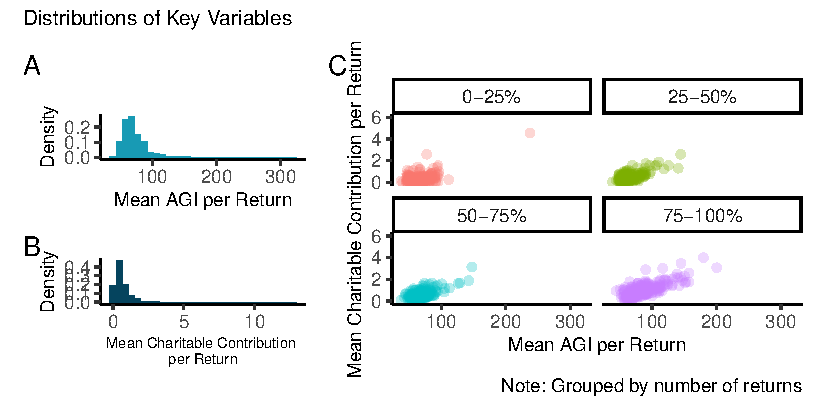
\includegraphics{Lab2_Assignment_files/figure-pdf/fig-dist-1.pdf}

}

\caption{\label{fig-dist}Panel (A) and (B) show the distribution of mean
AGI and mean charitable contribution respectively.In panel (C) we
present the joint distribution of the two, grouped by number of
returns.}

\end{figure}%

\paragraph{6. Model Specification}\label{model-specification}

We constructed a sequence of 4 main regression models, incrementally
adding theoretically relevant predictor variables to assess their impact
on the outcome variable, mean\_charitable\_contributation\_per\_return.
This sequential approach allows us to systematically examine the
influence of different economic factors on philanthropic behavior per
tax return.

Our model building process begins by establishing the core relationship
between income, as measured by mean\_agi\_per\_return, and charitable
contributions through several specifications. Model 1 examines a simple
linear relationship. Model 2 introduces a quadratic term for mean AGI to
capture potential non-linear effects. Model 3 explores a similar
non-linear relationship using the natural logarithm of mean AGI and its
squared term, to address the long-right tail shown from the distribution
plots above. Models 4 and 5 incorporate variables that proxy for wealth
and the availability of discretionary funds (mean dividend, mean cap
gain, and mean rent royalty), stable income sources (mean salary), and
tax-related variables (total net investment income tax amount and mean
tax payment).

\begin{table}[!htbp] \centering 
  \caption{Summary Table of the Models} 
  \label{} 
\tiny 
\begin{tabular}{@{\extracolsep{.001pt}}lcccc} 
\\[-1.8ex]\hline 
\hline \\[-1.8ex] 
 & \multicolumn{4}{c}{Dependent Variable: mean charitable contribution} \\ 
\cline{2-5} 
 & (1) & (2) & (4) & (5) \\ 
\hline \\[-1.8ex] 
 Mean AGI & 0.027$^{***}$ & 0.005$^{***}$ & 0.003$^{*}$ & $-$0.007 \\ 
  & (0.004) & (0.002) & (0.002) & (0.005) \\ 
  Mean AGI**2 &  & 0.0001$^{***}$ & 0.0001$^{***}$ & 0.0001$^{***}$ \\ 
  &  & (0.00000) & (0.00001) & (0.00002) \\ 
  Mean Dividend &  &  & 0.049$^{**}$ & 0.054$^{**}$ \\ 
  &  &  & (0.022) & (0.022) \\ 
  Mean Capgain &  &  & 0.004 & 0.006 \\ 
  &  &  & (0.003) & (0.004) \\ 
  Mean Rent Royalty &  &  & 0.001 & 0.003 \\ 
  &  &  & (0.004) & (0.004) \\ 
  Mean Salary &  &  &  & 0.012$^{**}$ \\ 
  &  &  &  & (0.005) \\ 
  Intercept & $-$1.316$^{***}$ & $-$0.240$^{***}$ & $-$0.335$^{***}$ & $-$0.371$^{*}$ \\ 
  & (0.303) & (0.089) & (0.116) & (0.191) \\ 
 \hline \\[-1.8ex] 
Observations & 2,089 & 2,089 & 2,089 & 2,089 \\ 
Adjusted R$^{2}$ & 0.602 & 0.706 & 0.785 & 0.790 \\ 
F Statistic & 3,156.028$^{***}$  & 2,512.758$^{***}$  & 1,526.683$^{***}$  & 1,313.285$^{***}$  \\ 
 & (df = 1; 2087) & (df = 2; 2086) & (df = 5; 2083) & (df = 6; 2082) \\
\hline 
\hline \\[-1.8ex] 
\textit{Note:}  & \multicolumn{4}{r}{$^{*}$p$<$0.1; $^{**}$p$<$0.05; $^{***}$p$<$0.01} \\ 
 & \multicolumn{4}{r}{Robust standard errors are displayed.} \\ 
 & \multicolumn{4}{r}{The covariate names omit per unit (e.g., per return) due to space limit.} \\ 
\end{tabular} 
\end{table}

\paragraph{7. Model Assumptions}\label{model-assumptions}

The first assumption for large-sample models is that the data is IID,
where each observation is independent from one another and that each
comes from the same distribution. The use of IRS Statistics of Income
(SOI) data presents some potential challenges to this IID assumption.
The raw data is aggregated at the ZIP code level, which inherently
introduces a degree of spatial dependence. While we normalize the data
by allocating the ZIP code level data to individual residential
addresses to reduce the impact of ZIP-level aggregation, observation
within the same county or neighboring areas may exhibit correlation from
shared socioeconomic or regional conditions which may violate the
independence assumption. Furthermore, while the IRS sampling process is
stratified, the underlying heterogeneity of individual tax returns may
still lead to concerns about the `identically distributed' aspect. For
instance, even within a county, the distribution of income and other
financial behaviors can vary. Additionally, our attempt to fix the issue
with identical distribution by excluding counties with less than 1,000
number of returns may reveal partial picture of the relationship between
the variables of our interest.

The second assumption is that a unique BLP should exist, where the
explanatory variables must have a finite mean and a finite, non-zero
variance, and that there is no perfect colinearity. Our visualizations
show that both of our main predictor and outcome variables have a heavy
right-tail, indicating a potential non-finite variance. We see that the
regression model runs, meaning that there is no perfect colinearity.
Although we see a non-infinite variance from our sample for exploration
(mean AGI: 4.82 , mean charitable contribution: 0.84 ), it should be
noted that the underlying distribution may still have non-finite
variance, which may violate our assumption for the presence of a unique
BLP.

\paragraph{8. Model Results and
Interpretation}\label{model-results-and-interpretation}

The regression models demonstrate a statistically significant
relationship between the predictor variables and mean charitable
contributions per return. All nine models are statistically significant
overall (p \textless{} 2.2e-16), indicating they explain a significant
portion of the variation in the dependent variable. The models vary in
their explanatory power, as measured by adjusted R-squared. Models 1 and
2 have lower adjusted R-squared values compared to Models 4 and 5,
indicating that including wealth/investment income and salary
significantly improves the model ability to explain charitable
contributions. Specifically, Model 1, which includes only mean AGI,
explains 60.2\% of the variation in charitable giving. Model 2 improves
upon this by adding a squared term for AGI, suggesting a non-linear
relationship, and increases the adjusted R-squared to 0.706. Models 4
and 5 further enhance the explanatory power. Model 4, which incorporates
wealth/investment income (mean dividend, capital gains, and rent/royalty
income), reaches an adjusted R-squared of 0.785, demonstrating the
importance of these factors in predicting charitable giving. Finally,
Model 5, with the inclusion of salary income, achieves an adjusted
R-squared of 0.790. This progression illustrates that charitable giving
is influenced by multiple factors, with income, wealth/investment
income, and salary all playing significant roles. Although subsequent
models (6 and 7) have slightly higher R-squared values, Model 5 may be a
better candidate due to its balance of explanatory power and parsimony.
See the appendix for details on Models 6 and 7.

A \$1,000 increase in mean salary is predicted to increase charitable
contributions by \$12, holding other variables constant. This suggests
that a \$10,000 increase in salary would lead to an additional \$120 in
predicted charitable giving, indicating a positive relationship between
salary and charitable donations. For every \$1,000 increase in mean
dividend income, charitable contributions are predicted to increase by
\$54 (coefficient = 0.054), suggesting individuals with higher dividend
earnings are, on average, expected to donate more, highlighting the
influence of investment income on charitable giving. Similarly, a
\$1,000 increase in mean capital gains is associated with a \$6 increase
in charitable contributions (coefficient = 0.006). This indicates that
capital gains also positively affect charitable giving. Finally, the
model captures a non-linear relationship between adjusted gross income
and charitable giving. At lower income levels (e.g., AGI of \$30,000),
the model might predict a smaller increase in charitable giving for each
additional \$1,000 of income, compared to someone with a high income
(e.g., AGI of \$100,000). For the higher-income individual, the model
predicts that each additional \$1,000 of income will lead to a more
substantial increase in charitable contributions. This pattern suggests
an U-shape relationship between AGI and charitable donations. The
coefficients for mean AGI and mean AGI squared are -0.007 and 0.0001
respectively. Mean rent royalty has a coefficient of 0.003.

\paragraph{9. Overall Effect}\label{overall-effect}

In a broader sense, these findings indicate that charitable giving is a
complex behavior influenced by a combination of factors. Stable income,
such as salary, and income from investments, such as dividends and
capital gains, both play a role. The non-linear effect of AGI suggests
that the propensity to donate changes as income levels vary. This has
implications for charitable organizations, which may tailor their
fundraising efforts to different income groups and those with different
sources of income.

\paragraph{References}\label{references}

\phantomsection\label{refs}
\begin{CSLReferences}{0}{1}
\end{CSLReferences}

\newpage

\subsection{Appendix}\label{appendix}

\subsubsection{1. Link to the Data
Source}\label{link-to-the-data-source}

\begin{itemize}
\item
  \url{https://www.irs.gov/statistics/soi-tax-stats-individual-income-tax-statistics-zip-code-data-soi}
\item
  \url{https://www.huduser.gov/apps/public/uspscrosswalk/login?previous=https://www.huduser.gov/apps/public/uspscrosswalk/home}
\item
  Link to the Google drive with the data sets downloaded from the sites
  above:
  \url{https://drive.google.com/drive/folders/12la_DQTyAJiNlq99ZdSQrpvSMdEPky5e?usp=sharing}
\end{itemize}

\subsubsection{2. List of the model
specifications}\label{list-of-the-model-specifications}

\begin{table}[!htbp] \centering 
  \caption{Summary Table of the Models Tried} 
  \label{} 
\tiny 
\begin{tabular}{@{\extracolsep{.001pt}}lcccccc} 
\\[-1.8ex]\hline 
\hline \\[-1.8ex] 
 & \multicolumn{6}{c}{Dependent Variable: mean charitable contribution} \\ 
\cline{2-7} 
 & (1) & (3) & (6) & (7) & (8) & (9) \\ 
\hline \\[-1.8ex] 
 Mean AGI & 0.027$^{***}$ &  & $-$0.008 & $-$0.007$^{*}$ &  &  \\ 
  & (0.004) &  & (0.005) & (0.004) &  &  \\ 
  & & & & & & \\ 
 Mean AGI**2 &  & $-$24.251$^{***}$ &  &  & $-$12.264$^{***}$ & $-$6.692$^{*}$ \\ 
  &  & (7.906) &  &  & (3.774) & (3.733) \\ 
  & & & & & & \\ 
 Log(Mean AGI) &  & 2.985$^{***}$ &  &  & 1.519$^{***}$ & 0.776$^{*}$ \\ 
  &  & (0.916) &  &  & (0.432) & (0.469) \\ 
  & & & & & & \\ 
 Log(Mean AGI**2) &  &  & 0.0001$^{***}$ & 0.0001$^{***}$ &  &  \\ 
  &  &  & (0.00002) & (0.00001) &  &  \\ 
  & & & & & & \\ 
 Mean Dividend &  &  & 0.055$^{**}$ & 0.056$^{**}$ & 0.056$^{***}$ & 0.055$^{*}$ \\ 
  &  &  & (0.022) & (0.028) & (0.017) & (0.029) \\ 
  & & & & & & \\ 
 Mean Capgain &  &  & 0.006 & 0.006 & 0.006 & 0.006 \\ 
  &  &  & (0.004) & (0.005) & (0.004) & (0.005) \\ 
  & & & & & & \\ 
 Mean Rent Royalty &  &  & 0.003 & 0.003 & 0.001 & 0.001 \\ 
  &  &  & (0.004) & (0.004) & (0.004) & (0.004) \\ 
  & & & & & & \\ 
 Mean Salary &  &  & 0.013$^{***}$ & 0.015$^{*}$ &  & 0.005 \\ 
  &  &  & (0.005) & (0.008) &  & (0.012) \\ 
  & & & & & & \\ 
 Total Net Investment &  &  & $-$0.00000 & $-$0.00000 &  & $-$0.00000 \\ 
  &  &  & (0.00000) & (0.00000) &  & (0.00000) \\ 
  & & & & & & \\ 
 Mean Tax Payment &  &  &  & $-$0.012 &  & 0.042 \\ 
  &  &  &  & (0.040) &  & (0.072) \\ 
  & & & & & & \\ 
 Intercept & $-$1.316$^{***}$ & 49.586$^{***}$ & $-$0.422$^{***}$ & $-$0.467$^{*}$ & 24.732$^{***}$ & 13.791$^{*}$ \\ 
  & (0.303) & (16.995) & (0.147) & (0.257) & (8.180) & (7.421) \\ 
  & & & & & & \\ 
\hline \\[-1.8ex] 
Observations & 2,089 & 2,089 & 2,089 & 2,089 & 2,089 & 2,089 \\ 
Adjusted R$^{2}$ & 0.602 & 0.644 & 0.792 & 0.792 & 0.762 & 0.770 \\ 
F Statistic & 3,156.028$^{***}$  & 1,891.352$^{***}$  & 1,135.563$^{***}$  & 994.457$^{***}$  & 1,339.826$^{***}$  & 872.358$^{***}$  \\ 
 & (df = 1; 2087) & (df = 2; 2086) & (df = 7; 2081) & (df = 8; 2080) & (df = 5; 2083) & (df = 8; 2080) \\
\hline 
\hline \\[-1.8ex] 
\textit{Note:}  & \multicolumn{6}{r}{$^{*}$p$<$0.1; $^{**}$p$<$0.05; $^{***}$p$<$0.01} \\ 
 & \multicolumn{6}{r}{Robust standard errors are displayed.} \\ 
 & \multicolumn{6}{r}{The covariate names omit per unit (e.g., per return) due to space limit.} \\ 
\end{tabular} 
\end{table}

Model uses log(mean AGI) and its squared term, also suggesting a
non-linear relationship between income and charitable giving, similar to
the findings in the main models. Both coefficients are statistically
significant. Because of the log transformation, the coefficients are
interpreted as elasticities. The adjusted R-squared of 0.644 indicates
that Model 3 explains 64.4\% of the variance in charitable giving,
showing that even when AGI is log-transformed, it remains a significant
predictor of donations.

Models 6, 7, 8, and 9 show that including wealth/investment, salary, and
tax-related variables further improves the model's ability to explain
charitable contributions, though some variables like rent royalty and
tax payments are not always significant. The adjusted R-squared values
for these models are:

Model 6 has an adjusted R-squared of 0.792 (indicating it explains
79.2\% of the variance). This shows that by adding more variables, the
explanatory power of the model increases compared to the earlier models.
Model 7 has an adjusted R-squared of 0.792 (indicating it also explains
79.2\% of the variance). This suggests that Model 7, with its specific
set of additional variables, explains a similar amount of variance as
Model 6. Model 8 uses log(mean AGI) and its squared term and has an
adjusted R-squared of 0.762 (indicating it explains 76.2\% of the
variance). This indicates that using the log of AGI in this model
results in slightly lower explanatory power than Models 6 and 7. Model 9
uses log(mean AGI) and its squared term, and also includes mean
dividend, mean campgain, mean rent royalty, and mean salary. It has an
adjusted R-squared of 0.770 (indicating it explains 77.0\% of the
variance). This shows that even with the inclusion of several income
variables, the model's explanatory power is still slightly lower than
Models 6 and 7.

\subsubsection{3. Residuals - vs - Fitted Values
Plots}\label{residuals---vs---fitted-values-plots}

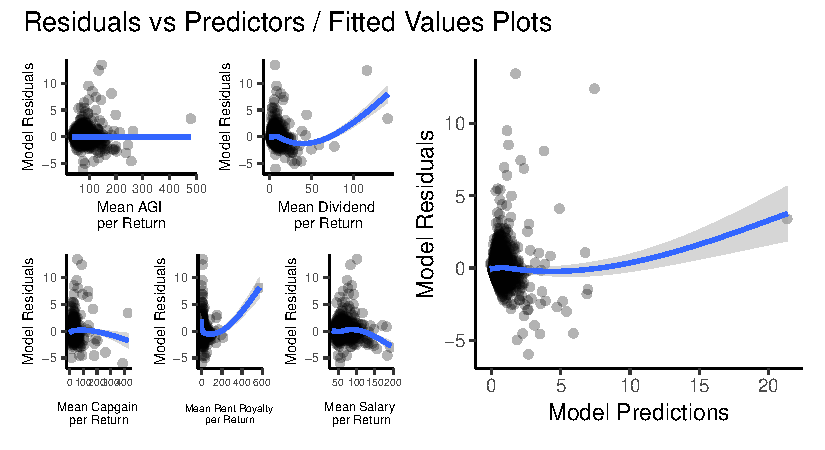
\includegraphics{Lab2_Assignment_files/figure-pdf/unnamed-chunk-6-1.pdf}




\end{document}
